\subsection{Descarte's Method of Tangents}

\subsubsection*{The Setup}

Prior to the differential calculus created by Leibniz and Newton, Descarte invented several methods of 
finding tangent lines to curves that are described by algebraic equations. These methods are purely
algebraic; they don't use either the concept of limits or infinitesimals. A nice reference on these
methods is Suzuki \cite{descarte}. Here we will discuss one of Descarte's simpler methods. As an example,
we will use Descarte's method to find the tangent line to the ellipse \(\{x^2 + 2y^2 = 3\}\) at the
point \((1,1)\).

To begin, let us define the two variable polynomail \(p(x,y) = x^2 + 2y^2 - 3\); we see that our ellipse is
the zero set \(\{p(x,y) = 0\} \).

Next, let us describe all of the non-vertical lines (not necessarily tangent lines) that pass through the 
point \((1,1)\). Consider any line \(y = mx + b\). If this line passes through \((1,1)\), then we have
\(1 = m + b\). So all of these lines are described by \(y = mx + 1 - m\) for different constants \(m\).

Next, let us observe that the interior of the ellipse is the set \(\{p(x,y) < 0\}\) and the exterior
is the set \(\{p(x,y) > 0\}\).
\begin{figure}[h]
\centering
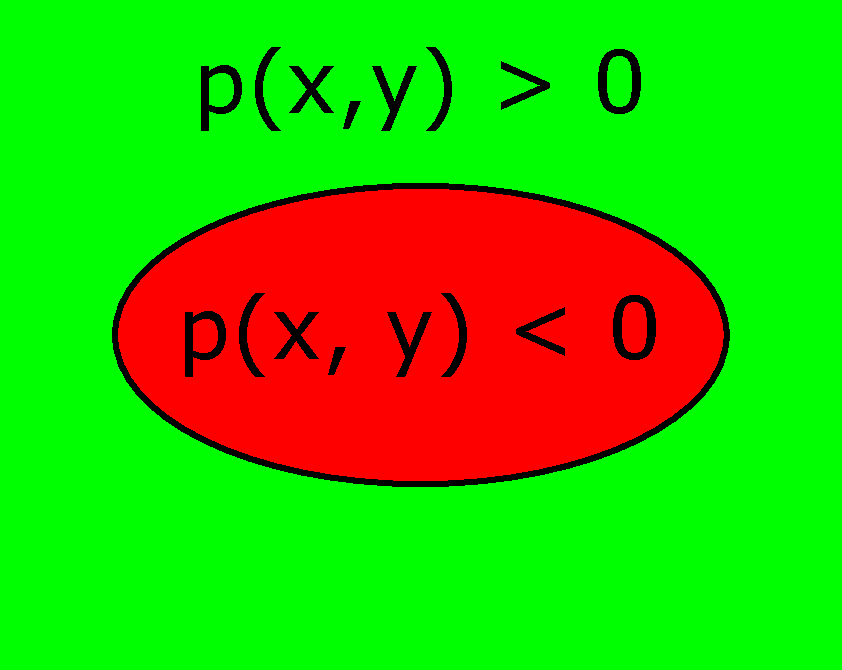
\includegraphics[width=2.5in]{preCalculus/signPoly.pdf}
\end{figure}

Next, let us see what the sign of \(p(x,y)\) looks like along different lines passing through \((1,1)\). 
When a line passing through \((1,1)\) is not a tangent line, close to \((1,1)\) the line passes through
both the interior and exterior of the ellipse. Therefore, for a non-tangent line, the sign of \(p(x,y)\)
changes. However, a tangent line will remain in the exterior of the ellipse (except at the point \((1,1)\)),
so \(p(x,y)\) will not change sign along the line. Consider the figure below.
\begin{figure}[h]
\centering
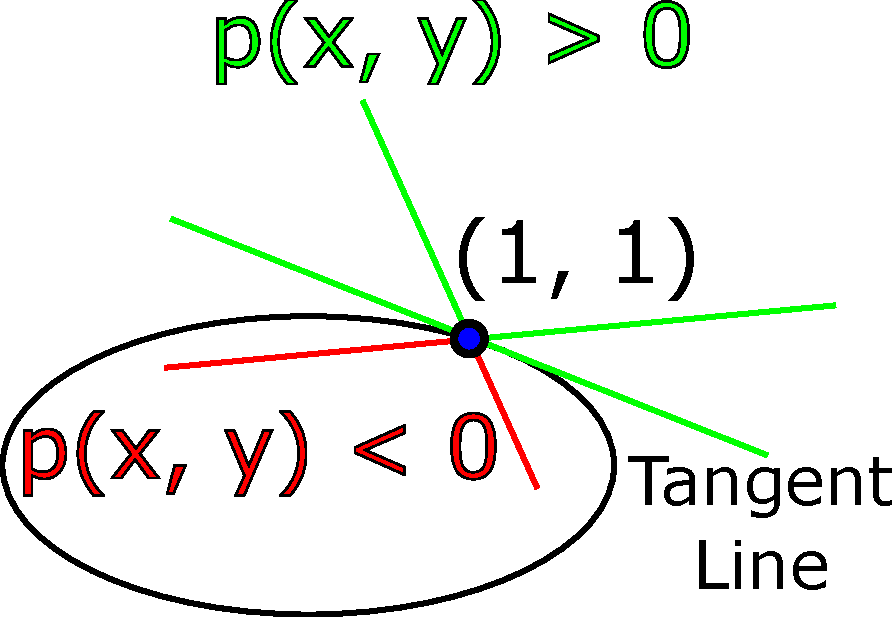
\includegraphics[width=2.5in]{preCalculus/signTangentLines.pdf}
\end{figure}  

So, given a line \(y = mx + 1 - m\) passing through \((1,1)\), let us compute the value of \(p(x,y\) along
the line. We parameterize this value by \(x\), so we have
\begin{align}
q(x) & \coloneqq p(x, mx + 1 - m), \\
    & = x^2 + 2(mx + 1 - m)^2 - 3, \\
    & = (1 + 2m^2)x^2 + 4(m - m^2) x + 2(1 - m)^2 - 3.
\end{align}

Now, we know that \(q(1) = 0\) since the line must intersect the ellipse at \((1,1)\). Futhermore, from our
argument above, we know that for non-tangent lines \(q(x)\) changes sign at \(x = 1\) and that the tangent
line must NOT change sign at \(q(x) = 1\).

Since the tangent line doesn't change sign, we know that for the correct value of the slope \(m\) for the
tangent line, the polynomial \(q(x)\) has a double root at \(x = 1\). Therefore, for the tangent line,
the polynomial is divisible by \((x - 1)^2 = x^2 - 2x + 1\); that is, after computing the polynomial division
\(\frac{q(x)}{x^2 - 2x + 1}\) we find a remainder of zero.

If we find that there is only one value of \(m\) that gives us a remainder of zero for this polynomial division,
then it must be the slope of the tangent line. Note that for non-tangent lines, we could also have that
\(q(x)\) is divisible by \((x - 1)^2\), since the sign will also change if there is a triple root.

\subsubsection*{The Problem}

Compute the slope of the tangent line \(y = mx + 1 -m\) passing through \((1,1)\) for the ellipse 
\(\{x^2 + 2y^2 = 3\}\) by finding the value of \(m\) for which the polynomial division
\begin{equation}
\frac{(1 + 2m^2)x^2 + 4(m - m^2)x + 2(1 - m)^2 - 3}{x^2 - 2x + 1},
\end{equation}
has vanishing remainder.

\subsubsection*{The Solution}

Let us perform the polynomial division.
\begin{align}
& \frac{(1 + 2m^2)x^2 + 4(m - m^2)x + 2(1 - m)^2 - 3}{x^2 - 2x + 1}, \\
= \, & 1 + 2m^2 + \frac{(2 + 4m^2 + 4m - 4m^2)x - 1 - 2m^2 + 2(1 - m)^2 - 3}{x^2 - 2x + 1}, \\ 
= \, & 1 + 2m^2 + \frac{(2 + 4m)x - 4m - 2 }{x^2 - 2x + 1}.
\end{align}
The degree of the numerator is less than the denominator, so the numerator is the remainder. Therefore,
we must have that \((2 + 4m)x - 4m - 2 = 0\). So the coefficients must vanish and we get
\begin{equation}
\begin{cases}
2 + 4m = 0, \\
-4m - 2 = 0.
\end{cases}
\end{equation}
The system has the unique solution \(m = -1/2\); therefore the slope of the tangent line must be \(m = -1/2\).
So we find the tangent line to be
\begin{equation}
y = -\frac{1}{2}x + \frac{3}{2}.
\end{equation}
